\newpage
\section{Analysis}

Each feature of the word-vector model obtains its co-efficients from two separate sources:
\begin{itemize}
\item the first set of weights are trained in a similar fashion to the vanilla logistic regression model
\item the second set of weights are learnt by enforcing a word-vector regularization
\end{itemize}

We train the model as follows:\\

We initially keep word-vector weights constant at zero.
We then find the best model performance by training only the vanilla logistic regression model through extensive hyper-parameter tuning (l1/l2 regularization).

Once the vanilla feature weights have been learnt, we then start learning the word-vectors weights by increasing the l1/l2 regularization on the vanilla feature weights. This regularization would force the model to reduce the strength of the vanilla weights and move them to the unregularized word-vector weights. As the l1/l2 regularization strength per feature starts increasing, more and more weight from the vanilla model starts to shift onto the word-vector feature weights. 
The word-vector weights are constrained by a word-vector function. So when the word-vector model weights are substantial enough, then due to the word-vector similarity property, we are able to see the weights of the rare similar words also to start having a higher weight. This boosting of the rare word-weights would help improving the performance of the model.

However it is also possible that some labels better perform using the vanilla weights rather than the word-vector weights. In such a case, applying high regularization on the vanilla weights to boost the word-vector weights would be counterproductive. Thus, we need to perform extensive hyper-parameter tuning to find the right set of vanilla and word-vector weights that would work on all kinds of labels.\\

We performed several experiments to find the right set of hyper-parameters. Through these experiments we noticed that if the l1 penalty on the vanilla weights was too low, then the word-vector weights wouldn't increase much at all. They would remain almost close to zero. As we applied more and more l1 penalty, the model was forced to learn through the word-vector weights. 

Below is a graph showing various test results comparing l1 constraint per feature versus word-vector weights. We can see that the word-vector weights were increasing with higher L1 up to a certain point. After a certain threshold, the word-vector weights were almost non-increasing.

We also compared the model performance vs L1 strength. We can clearly see that the model performance increases initially with increasing L1 regularization and after a certain threshold, we see the model performance start to go down.\\\\

\begin{figure}[htbp]
\centering
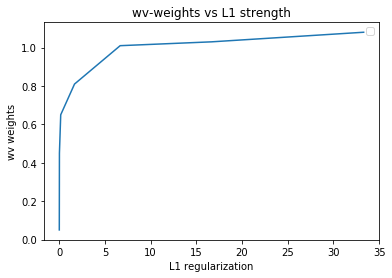
\includegraphics[width=16cm, height=10cm]{images/graph1.png}\\
\centering
\caption{Graph comparing word-vector weights with increasing L1 regularization}
\label{fig:graph1}
\end{figure}

\begin{figure}[htbp]
\centering
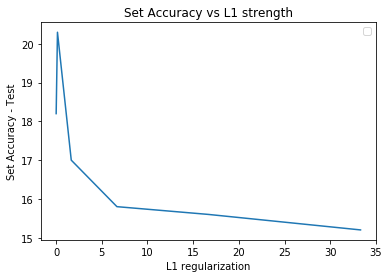
\includegraphics[width=16cm, height=10cm]{images/graph2.png}\\
\centering
\caption{Graph comparing model performance with increasing L1 regularization}
\label{fig:graph2}
\end{figure}


Upon comparing both models, we noticed that the performance of the word-vector models improved due to the additional word-vector weights.

To verify this, we took the top features for each model and printed the following:

\begin{itemize}
\item top similar words for each feature calculated based on the cosine similarity of the word-vectors

\item cosine similarity of the similar word

\item feature weight of the similar word

\item idf score of the similar word
\end{itemize}

The idf scores were computed to measure the rarity of the words. We noticed that the rare features which were similar to the important features now had similar weights. The below section shows such examples:

\subsection{Examples of rare-similar words now having similar weights}

In this section we show a few examples where the word-vector model is able to generate similar weights for similar words, even if some of these words are rare. The rarity of the word can be determined by their corresponding Idf score. Due to the rarity of the words, the vanilla logistic regression model did not have enough information to determine the influence of these rare words and assigned them very small weights. However the word-vector models were able to assign comparatively higher weights due to their similarity feature. \\

In the below example, we can see that \textbf{marijuana} and \textbf{narcotics} are rare features based on their higher Idf scores. Inspite of that, due to their similarity with the \textbf{drug}, they have substantially higher word-vector weights. Comparatively these rare words have very small weights when trained through vanilla logistic regression model. Thus, after using the word-vector model, when these rare words do appear in the test set, they now have a higher chance of getting classified under the class \textbf{Drug}.

\begin{table}[htbp]
\begin{tabular}{llllll}
\multicolumn{2}{l|}{\textbf{Class: Drug}}                                  & \multicolumn{1}{l|}{\textbf{\begin{tabular}[c]{@{}l@{}}vanilla\\ weights\end{tabular}}} & \multicolumn{1}{l|}{\textbf{Similarity}} & \multicolumn{1}{l|}{\textbf{Idf-score}} & \textbf{\begin{tabular}[c]{@{}l@{}}wv\\ weights\end{tabular}} \\ \hline
\multicolumn{1}{l|}{\textbf{Top-feature}} & \multicolumn{1}{l|}{cannabis}  & \multicolumn{1}{l|}{0.388}                                                              & \multicolumn{1}{l|}{1}                   & \multicolumn{1}{l|}{5.5}                & 0.159                                                         \\ \hline
\multicolumn{1}{l|}{\textbf{Top similar}} & \multicolumn{1}{l|}{marijuana} & \multicolumn{1}{l|}{0.012}                                                              & \multicolumn{1}{l|}{0.764}               & \multicolumn{1}{l|}{6}                  & 0.126                                                         \\
\multicolumn{1}{l|}{\textbf{features}}    & \multicolumn{1}{l|}{heroin}    & \multicolumn{1}{l|}{0.097}                                                              & \multicolumn{1}{l|}{0.694}               & \multicolumn{1}{l|}{4.86}               & 0.129                                                         \\
\multicolumn{1}{l|}{}                     & \multicolumn{1}{l|}{narcotics} & \multicolumn{1}{l|}{-2e-5}                                                              & \multicolumn{1}{l|}{0.557}               & \multicolumn{1}{l|}{6.19}               & 0.06                                                          \\
                                          &                                &                                                                                         &                                          &                                         &                                                              
\end{tabular}
\caption{\label{tab:widgets}Top feature weights comparison for Drugs}
\end{table}

\newpage

Here is an example which displays the vanilla and word-vector model weights for \textbf{chinese}, \textbf{shanghai} and \textbf{taiwan} which are some of the words used in similar context to \textbf{beijing}. Since \textbf{chinese} is not a rare word, we can see that its vanilla logistic regression model weight is quite high as compared to the word-vector model weight. However, when it comes across rarer words like \textbf{shanghai} and \textbf{taiwan}, its corresponding vanilla weights have dropped significantly, whereas the word-vector model weights are comparatively higher and closer to their corresponding word-vector weight of \textbf{beijing}.

\begin{table}[htbp]
\begin{tabular}{llllll}
\multicolumn{2}{l|}{\textbf{Class: China}}                                & \multicolumn{1}{l|}{\textbf{\begin{tabular}[c]{@{}l@{}}vanilla\\ weights\end{tabular}}} & \multicolumn{1}{l|}{\textbf{Similarity}} & \multicolumn{1}{l|}{\textbf{Idf-score}} & \textbf{\begin{tabular}[c]{@{}l@{}}wv\\ weights\end{tabular}} \\ \hline
\multicolumn{1}{l|}{\textbf{Top-feature}} & \multicolumn{1}{l|}{beijing}  & \multicolumn{1}{l|}{0.252}                                                              & \multicolumn{1}{l|}{1}                   & \multicolumn{1}{l|}{4.01}               & 0.215                                                         \\ \hline
\multicolumn{1}{l|}{\textbf{Top similar}} & \multicolumn{1}{l|}{chinese}  & \multicolumn{1}{l|}{0.376}                                                              & \multicolumn{1}{l|}{0.696}               & \multicolumn{1}{l|}{3.23}               & 0.166                                                         \\
\multicolumn{1}{l|}{\textbf{features}}    & \multicolumn{1}{l|}{shanghai} & \multicolumn{1}{l|}{0.075}                                                              & \multicolumn{1}{l|}{0.656}               & \multicolumn{1}{l|}{5.17}               & 0.10                                                          \\
\multicolumn{1}{l|}{}                     & \multicolumn{1}{l|}{taiwan}   & \multicolumn{1}{l|}{3e-5}                                                               & \multicolumn{1}{l|}{0.607}               & \multicolumn{1}{l|}{5.53}               & 0.073                                                         \\
                                          &                               &                                                                                         &                                          &                                         &                                                              
\end{tabular}
\caption{\label{tab:widgets}Top feature weights comparison for China}
\end{table}

Below is a similar example where \textbf{ranch} is a top feature for the class \textbf{Western}. Again we can see that the weights of rare-words \textbf{cattle}, \textbf{farm} and \textbf{sheep} have been boosted due to the word-vector model.

\begin{table}[htbp]
\begin{tabular}{llllll}
\multicolumn{2}{l|}{\textbf{Class: Western}}                             & \multicolumn{1}{l|}{\textbf{\begin{tabular}[c]{@{}l@{}}vanilla\\ weights\end{tabular}}} & \multicolumn{1}{l|}{\textbf{Similarity}} & \multicolumn{1}{l|}{\textbf{Idf-score}} & \textbf{\begin{tabular}[c]{@{}l@{}}wv\\ weights\end{tabular}} \\ \hline
\multicolumn{1}{l|}{\textbf{Top-feature}} & \multicolumn{1}{l|}{ranch}  & \multicolumn{1}{l|}{0.103}                                                              & \multicolumn{1}{l|}{1}                   & \multicolumn{1}{l|}{5.29}               & 1.216                                                         \\ \hline
\multicolumn{1}{l|}{\textbf{Top similar}} & \multicolumn{1}{l|}{cattle} & \multicolumn{1}{l|}{0.050}                                                              & \multicolumn{1}{l|}{0.716}               & \multicolumn{1}{l|}{5.55}               & 0.878                                                         \\
\multicolumn{1}{l|}{\textbf{features}}    & \multicolumn{1}{l|}{farm}   & \multicolumn{1}{l|}{-4e-5}                                                               & \multicolumn{1}{l|}{0.705}               & \multicolumn{1}{l|}{4.24}               & 0.486                                                         \\
\multicolumn{1}{l|}{}                     & \multicolumn{1}{l|}{sheep}  & \multicolumn{1}{l|}{-3e-5}                                                               & \multicolumn{1}{l|}{0.591}               & \multicolumn{1}{l|}{6.03}               & 0.314                                                         \\
                                          &                             &                                                                                         &                                          &                                         &                                                              
\end{tabular}
\caption{\label{tab:widgets}Top feature weights comparison for West}
\end{table}

The above examples do help in proving that our model was successfully able to use word-vectors as a regularizer to assign similar weights to similar words even if those similar words happen to be rare.

\newpage
\subsection{Scenarios when word-vector model doesn't work}

\begin{table}[htbp]
\begin{tabular}{llllll}
\multicolumn{2}{l|}{\textbf{Class: Western}}                           & \multicolumn{1}{l|}{\textbf{\begin{tabular}[c]{@{}l@{}}vanilla\\ weights\end{tabular}}} & \multicolumn{1}{l|}{\textbf{Similarity}} & \multicolumn{1}{l|}{\textbf{Idf-score}} & \textbf{\begin{tabular}[c]{@{}l@{}}wv\\ weights\end{tabular}} \\ \hline
\multicolumn{1}{l|}{\textbf{Top-feature}} & \multicolumn{1}{l|}{west}  & \multicolumn{1}{l|}{0.224}                                                              & \multicolumn{1}{l|}{1}                   & \multicolumn{1}{l|}{3.95}               & 0.981                                                         \\ \hline
\multicolumn{1}{l|}{\textbf{Top similar}} & \multicolumn{1}{l|}{north} & \multicolumn{1}{l|}{-4e-5}                                                              & \multicolumn{1}{l|}{0.823}               & \multicolumn{1}{l|}{4.06}               & 0.38                                                          \\
\multicolumn{1}{l|}{\textbf{features}}    & \multicolumn{1}{l|}{east}  & \multicolumn{1}{l|}{-3e-5}                                                              & \multicolumn{1}{l|}{0.822}               & \multicolumn{1}{l|}{4.26}               & 0.297                                                         \\
\multicolumn{1}{l|}{}                     & \multicolumn{1}{l|}{south} & \multicolumn{1}{l|}{5e-5}                                                               & \multicolumn{1}{l|}{0.821}               & \multicolumn{1}{l|}{3.72}               & 0.232                                                         \\
                                          &                            &                                                                                         &                                          &                                         &                                                              
\end{tabular}
\end{table}

\subsection{Scenarios when word-vector model works because of word-vector coefficients not because of similarity}

\begin{table}[htbp]
\begin{tabular}{llllll}
\multicolumn{2}{l|}{\textbf{Class: Brazil}}                                 & \multicolumn{1}{l|}{\textbf{\begin{tabular}[c]{@{}l@{}}vanilla\\ weights\end{tabular}}} & \multicolumn{1}{l|}{\textbf{Similarity}} & \multicolumn{1}{l|}{\textbf{Idf-score}} & \textbf{\begin{tabular}[c]{@{}l@{}}wv\\ weights\end{tabular}} \\ \hline
\multicolumn{1}{l|}{\textbf{Top-feature}} & \multicolumn{1}{l|}{amazon}     & \multicolumn{1}{l|}{0.086}                                                              & \multicolumn{1}{l|}{1}                   & \multicolumn{1}{l|}{4.3}                & 0.146                                                         \\ \hline
\multicolumn{1}{l|}{\textbf{Top similar}} & \multicolumn{1}{l|}{kindle}     & \multicolumn{1}{l|}{-4e-5}                                                              & \multicolumn{1}{l|}{0.699}               & \multicolumn{1}{l|}{5.96}               & 0.037                                                         \\
\multicolumn{1}{l|}{\textbf{features}}    & \multicolumn{1}{l|}{ebooks}     & \multicolumn{1}{l|}{-1e-5}                                                              & \multicolumn{1}{l|}{0.655}               & \multicolumn{1}{l|}{6.51}               & 0.004                                                         \\
\multicolumn{1}{l|}{}                     & \multicolumn{1}{l|}{rainforest} & \multicolumn{1}{l|}{1e-5}                                                               & \multicolumn{1}{l|}{0.521}               & \multicolumn{1}{l|}{5.32}               & 0.13                                                          \\
                                          &                                 &                                                                                         &                                          &                                         &                                                              
\end{tabular}
\end{table}

\begin{table}[htbp]
\begin{tabular}{llllll}
\multicolumn{2}{l|}{\textbf{Class: Crime}}                                   & \multicolumn{1}{l|}{\textbf{\begin{tabular}[c]{@{}l@{}}vanilla\\ weights\end{tabular}}} & \multicolumn{1}{l|}{\textbf{Similarity}} & \multicolumn{1}{l|}{\textbf{Idf-score}} & \textbf{\begin{tabular}[c]{@{}l@{}}wv\\ weights\end{tabular}} \\ \hline
\multicolumn{1}{l|}{\textbf{Top-feature}} & \multicolumn{1}{l|}{examination} & \multicolumn{1}{l|}{1.5}                                                                & \multicolumn{1}{l|}{1}                   & \multicolumn{1}{l|}{5.63}               & 0.245                                                         \\ \hline
\multicolumn{1}{l|}{\textbf{Top similar}} & \multicolumn{1}{l|}{tests}       & \multicolumn{1}{l|}{1e-4}                                                               & \multicolumn{1}{l|}{0.698}               & \multicolumn{1}{l|}{5.53}               & 0.003                                                         \\
\multicolumn{1}{l|}{\textbf{features}}    & \multicolumn{1}{l|}{exam}        & \multicolumn{1}{l|}{1e-5}                                                               & \multicolumn{1}{l|}{0.646}               & \multicolumn{1}{l|}{6.55}               & 0.010                                                         \\
\multicolumn{1}{l|}{}                     & \multicolumn{1}{l|}{analysis}    & \multicolumn{1}{l|}{0.496}                                                              & \multicolumn{1}{l|}{0.642}               & \multicolumn{1}{l|}{6.93}               & 0.21                                                          \\
                                          &                                  &                                                                                         &                                          &                                         &                                                              
\end{tabular}
\end{table}